\subsection{Modelo M/M/1 en Python}

Para analizar el rendimiento del modelo, variamos la tasa de arribos ($T_a$) en base a la tasa de servicio ($T_s$), y
la capacidad de la cola ($cap$).

Realizaremos 100 simulaciones de 1000 clientes cada una y promediamos los siguientes estadísticos:
\begin{itemize}
    \item Promedio de clientes en el sistema ($q(n)+u(n)$)
    \item Cantidad de clientes en cola en promedio ($q(n)$)
    \item Demora promedio esperada en cola ($d(n)$)
    \item Tiempo promedio en el sistema ($d(n)+s(n)$)
    \item Ocupación del servidor ($u(n)$)
    \item Probabilidad de denegación del servicio. ($p(den)$)
    \item Probabilidad de encontrar n clientes en cola. ($p(Q(t)=n)$)
\end{itemize}

Presentaremos los resultados obtenidos junto con sus intervalos de confianza del 95\%, obtenidos suponiendo que los mismos se distribuyen de manera normal, por el teorema central del límite, en el formato $valor \pm error$.

\subsubsection[cap = 0]{$cap = 0$}

Los parámetros $d(n)$, $q(n)$ y $p(Q(t)=n)$ no aplican cuando la capacidad de la cola es 0. El promedio de clientes en sistema es en este caso, equivalente al factor de uso del servicio.

\begin{tabular}{||c||c|c|c||}
    \hline \hline
    $\frac{T_a}{T_s}\times100\%$ [\%] & $d(n)+s(n)$ [min] & $u(n)\times100\%$ [\%] & $p(den)$ [\%] \\
    \hline \hline
    25 & $1.992 \pm 0.122$ & $19.915 \pm 1.375$ & $19.878 \pm 2.118$ \\
    \hline
    50 & $2.003 \pm 0.126$ & $33.32 \pm 1.803$ & $33.354 \pm 2.358$ \\
    \hline
    75 & $2.004 \pm 0.119$ & $42.924 \pm 2.14$ & $42.892 \pm 2.048$ \\
    \hline
    100 & $1.991 \pm 0.116$ & $49.905 \pm 2.116$ & $49.596 \pm 2.279$ \\
    \hline
    125 & $2.008 \pm 0.122$ & $55.555 \pm 2.066$ & $55.503 \pm 2.028$ \\
    \hline \hline
\end{tabular}

\subsubsection[cap = 2]{$cap = 2$}

\begin{small}
  \begin{tabular}{||c||c|c|c|c|c|c||}
    \hline \hline
    $\frac{T_a}{T_s}\times100\%$ [\%] & $q(n)+u(n)$ [min] & $q(n)$ [clientes] & $d(n)$ [min] & $d(n)+s(n)$ [min] & $u(n)\times100\%$ [\%] & $p(den)$ [\%] \\
    \hline \hline
    25 & $0.32 \pm 0.031$ & $0.071 \pm 0.015$ & $0.576 \pm 0.112$ & $2.589 \pm 0.198$ & $24.871 \pm 1.842$ & $1.165 \pm 0.811$ \\
    \hline
    50 & $0.737 \pm 0.082$ & $0.269 \pm 0.049$ & $1.15 \pm 0.207$ & $3.154 \pm 0.337$ & $46.817 \pm 3.684$ & $6.666 \pm 2.297$ \\
    \hline
    75 & $1.141 \pm 0.102$ & $0.51 \pm 0.069$ & $1.604 \pm 0.225$ & $3.593 \pm 0.347$ & $63.133 \pm 3.754$ & $15.088 \pm 3.029$ \\
    \hline
    100 & $1.507 \pm 0.119$ & $0.754 \pm 0.085$ & $2.006 \pm 0.25$ & $4.009 \pm 0.368$ & $75.238 \pm 3.781$ & $25.061 \pm 3.607$ \\
    \hline
    125 & $1.773 \pm 0.1$ & $0.946 \pm 0.075$ & $2.282 \pm 0.239$ & $4.278 \pm 0.351$ & $82.628 \pm 2.868$ & $33.783 \pm 3.5$ \\
    \hline \hline
  \end{tabular}
\end{small}

\begin{figure}[H]
  \centering
  \begin{subfigure}{0.267\linewidth}
    \importarcontenidofigura{cola_mm1_2_25_probabilidad_n_clientes}
  \end{subfigure}\hspace{0.35cm}
  \begin{subfigure}{0.267\linewidth}
    \importarcontenidofigura{cola_mm1_2_50_probabilidad_n_clientes}
  \end{subfigure}\hspace{0.35cm}
  \begin{subfigure}{0.267\linewidth}
    \importarcontenidofigura{cola_mm1_2_75_probabilidad_n_clientes}
  \end{subfigure}
  \begin{subfigure}{0.267\linewidth}
    \importarcontenidofigura{cola_mm1_2_100_probabilidad_n_clientes}
  \end{subfigure}\hspace{0.35cm}
  \begin{subfigure}{0.267\linewidth}
    \importarcontenidofigura{cola_mm1_2_125_probabilidad_n_clientes}
  \end{subfigure}
  \caption{Probabilidad de encontrar n clientes en cola, con bandas de error del 95\%.}
\end{figure}

\subsubsection[cap = 5]{$cap = 5$}

\begin{tabular}{||c||c|c|c|c|c|c||}
    \hline \hline
    $\frac{T_a}{T_s}\times100\%$ [\%] & $q(n)+u(n)$ [min] & $q(n)$ [clientes] & $d(n)$ [min] & $d(n)+s(n) [min]$ & $u(n)\times100\%$ [\%] & $p(den)$ [\%] \\
    \hline \hline
    25 & $$ & $$ & $$ & $$ & $$ & $$ \\
    \hline
    50 & $$ & $$ & $$ & $$ & $$ & $$ \\
    \hline
    75 & $$ & $$ & $$ & $$ & $$ & $$ \\
    \hline
    100 & $$ & $$ & $$ & $$ & $$ & $$ \\
    \hline
    125 & $$ & $$ & $$ & $$ & $$ & $$ \\
    \hline \hline
\end{tabular}

\begin{figure}[H]
  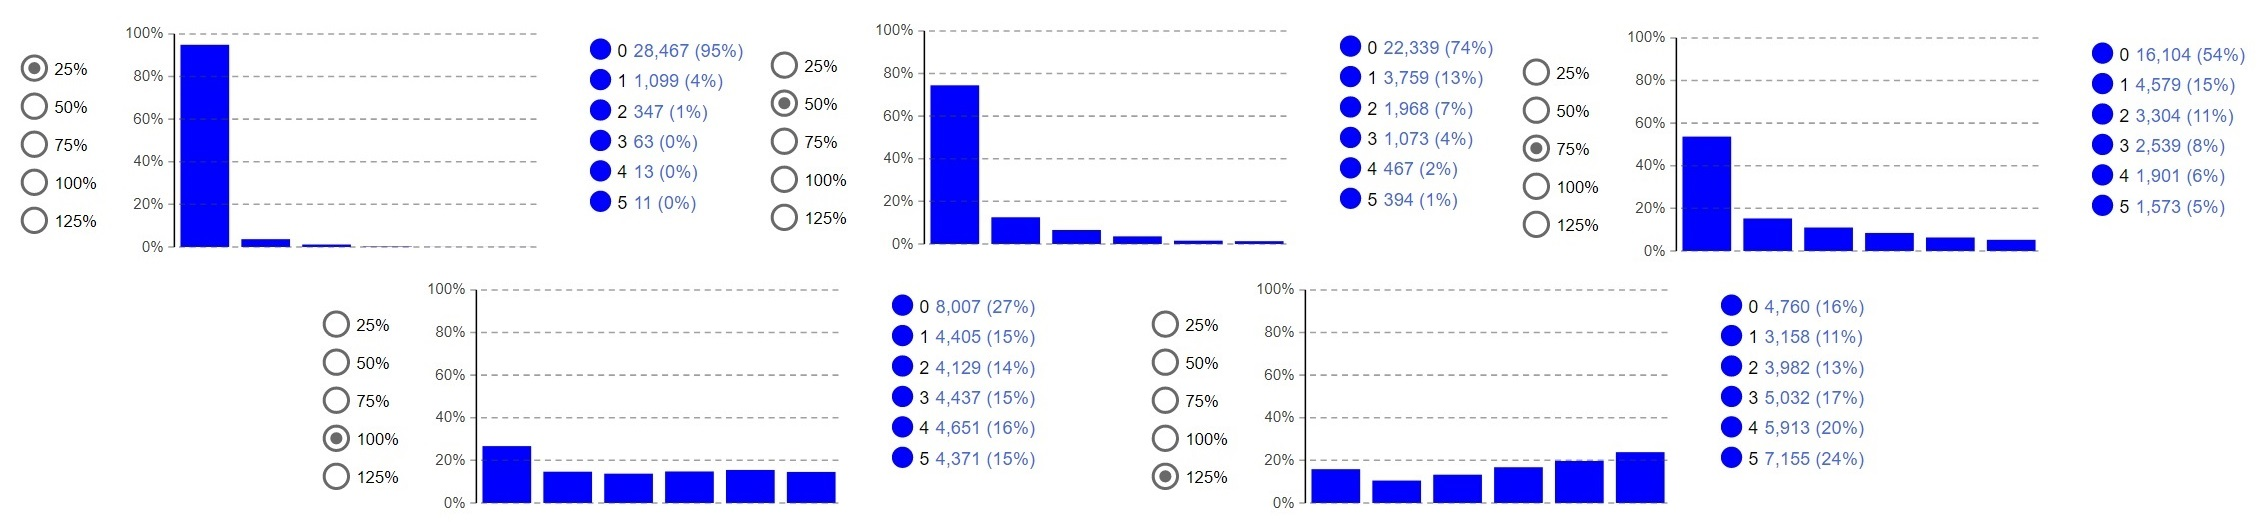
\includegraphics[width=\linewidth]{images/anylogic-colas-5}
  \caption{Probabilidad de encontrar n clientes en cola.}
\end{figure}

\subsubsection[cap = 10]{$cap = 10$}

\begin{tabular}{||c||c|c|c|c|c|c||}
    \hline \hline
    $\frac{T_a}{T_s}\times100\%$ [\%] & $q(n)+u(n)$ [min] & $q(n)$ [clientes] & $d(n)$ [min] & $d(n)+s(n) [min]$ & $u(n)\times100\%$ [\%] & $p(den)$ [\%] \\
    \hline \hline
    25 & $$ & $$ & $$ & $$ & $$ & $$ \\
    \hline
    50 & $$ & $$ & $$ & $$ & $$ & $$ \\
    \hline
    75 & $$ & $$ & $$ & $$ & $$ & $$ \\
    \hline
    100 & $$ & $$ & $$ & $$ & $$ & $$ \\
    \hline
    125 & $$ & $$ & $$ & $$ & $$ & $$ \\
    \hline \hline
\end{tabular}

\begin{figure}[H]
  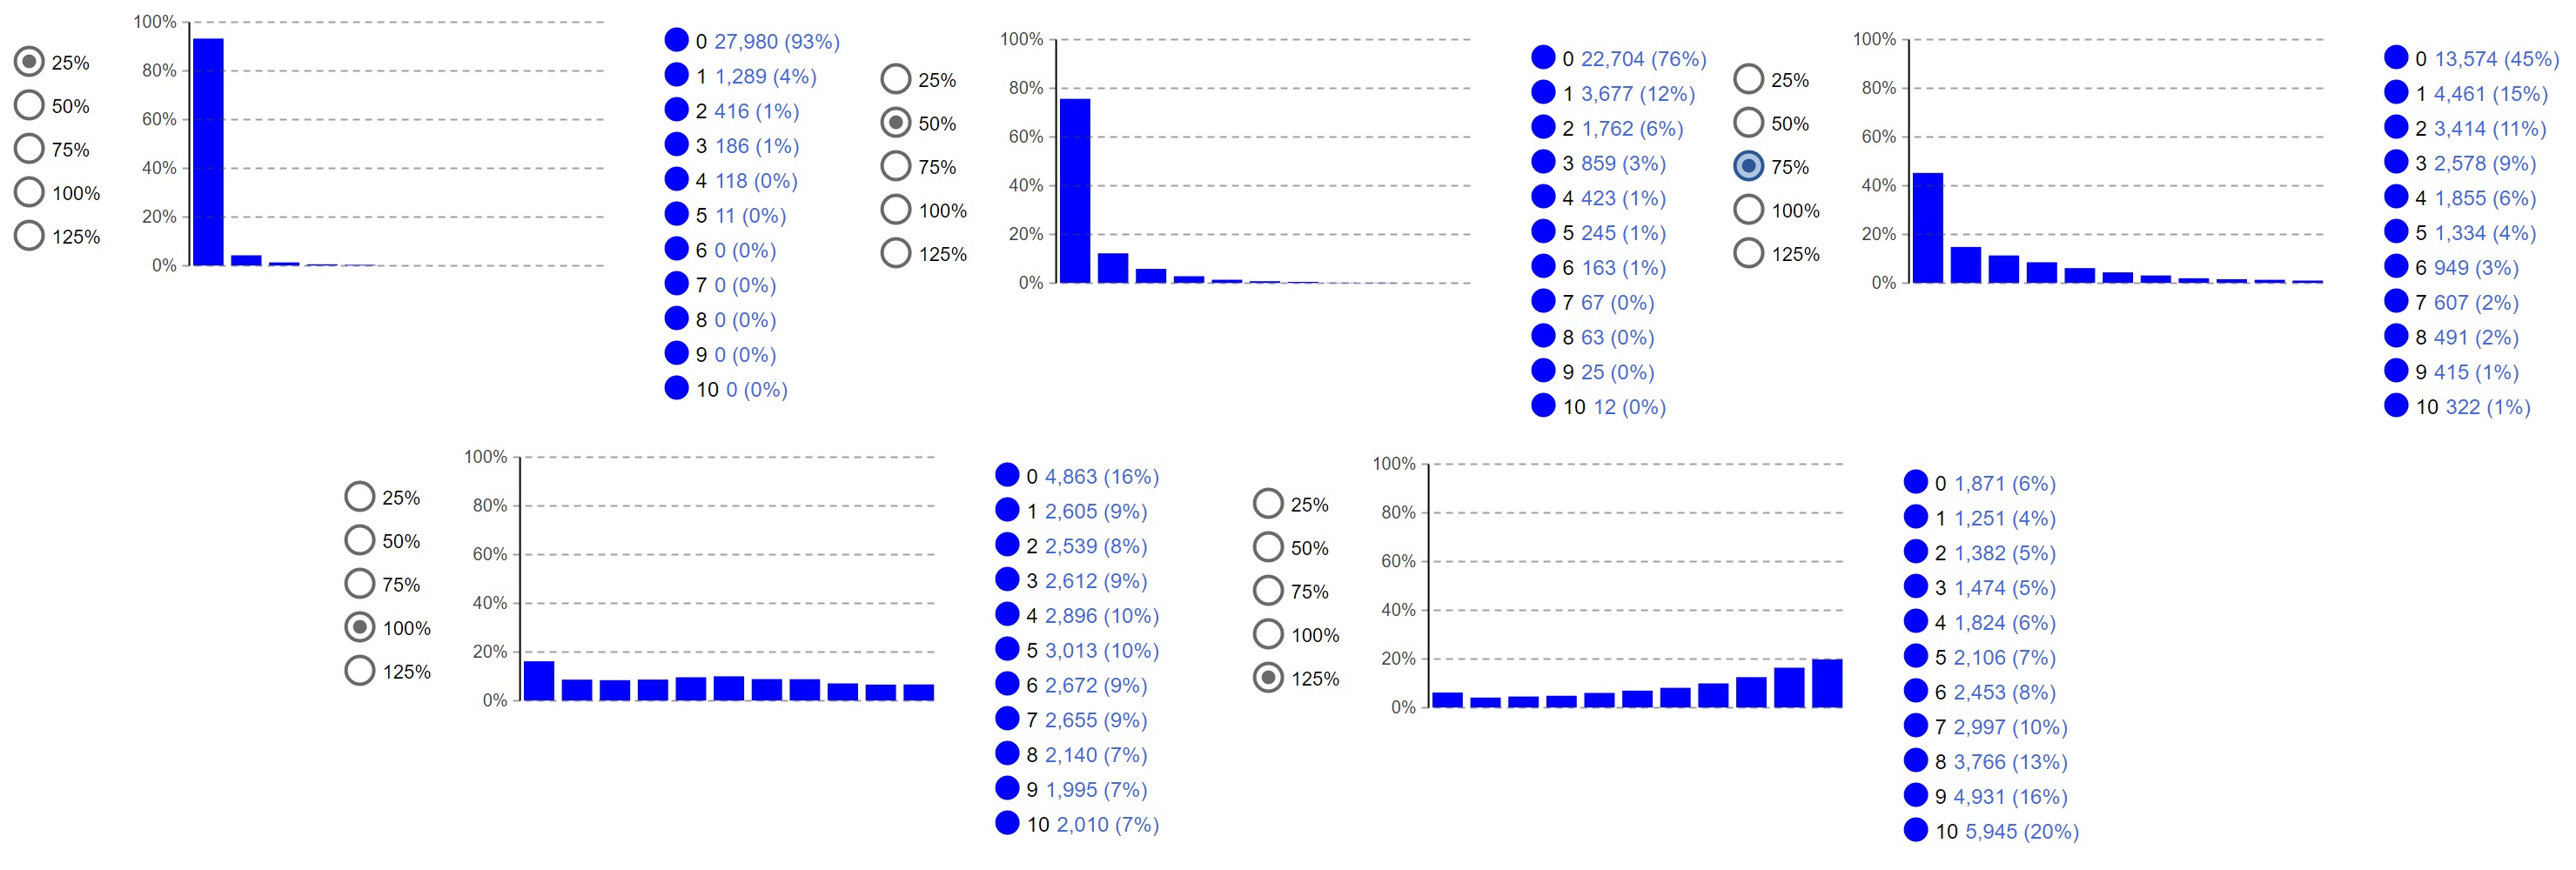
\includegraphics[width=\linewidth]{images/anylogic-colas-10}
  \caption{Probabilidad de encontrar n clientes en cola.}
\end{figure}

\subsubsection[cap = 50]{$cap = 50$}

\begin{tabular}{||c||c|c|c|c|c|c||}
    \hline \hline
    $\frac{T_a}{T_s}\times100\%$ [\%] & $q(n)+u(n)$ [min] & $q(n)$ [clientes] & $d(n)$ [min] & $d(n)+s(n) [min]$ & $u(n)\times100\%$ [\%] & $p(den)$ [\%] \\
    \hline \hline
    25 & $$ & $$ & $$ & $$ & $$ & $$ \\
    \hline
    50 & $$ & $$ & $$ & $$ & $$ & $$ \\
    \hline
    75 & $$ & $$ & $$ & $$ & $$ & $$ \\
    \hline
    100 & $$ & $$ & $$ & $$ & $$ & $$ \\
    \hline
    125 & $$ & $$ & $$ & $$ & $$ & $$ \\
    \hline \hline
\end{tabular}

\begin{figure}[H]
  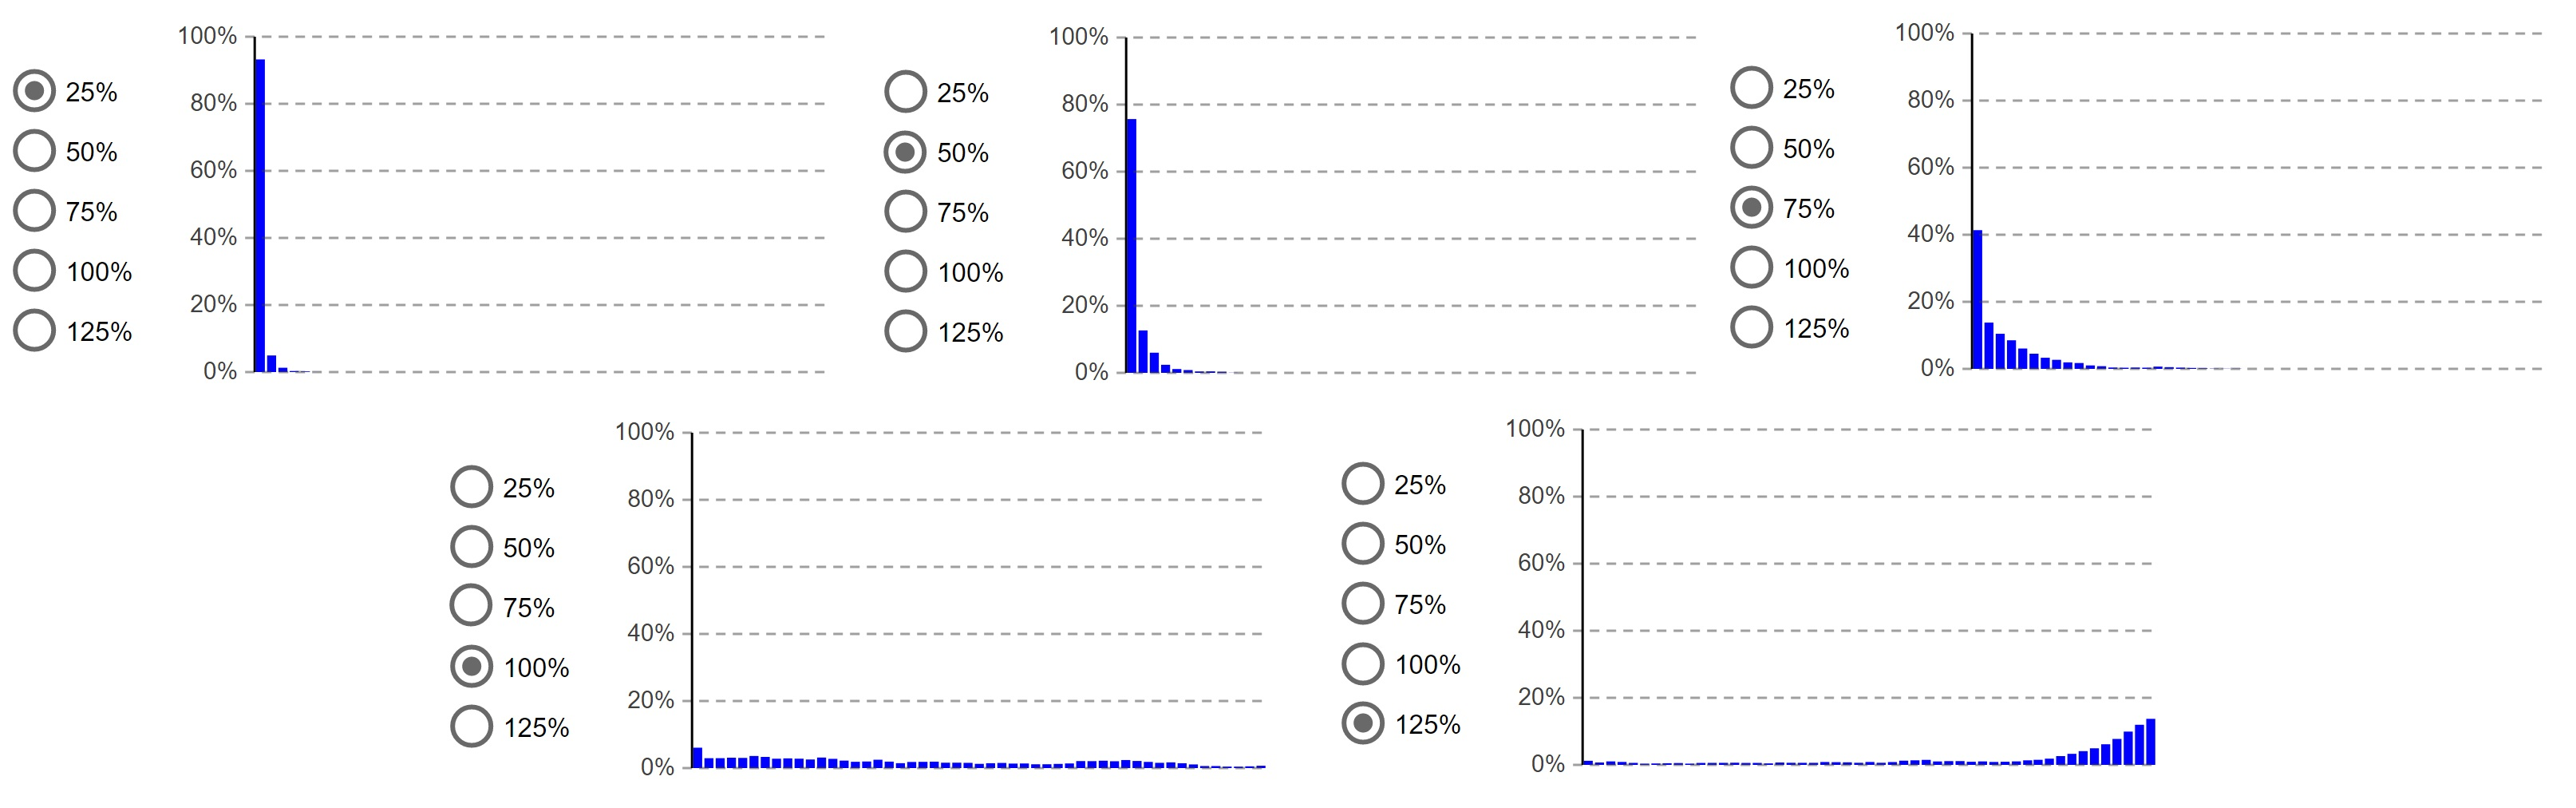
\includegraphics[width=\linewidth]{images/anylogic-colas-50}
  \caption{Probabilidad de encontrar n clientes en cola.}
\end{figure}

\subsubsection[cap = ∞]{$cap = \infty$}

En este caso no tenemos tope de clientes en la cola, entonces no hay probabilidad de denegación.

\begin{itemize}
    \item Promedio de clientes en el sistema ($q(n)+u(n)$)
    \item Cantidad de clientes en cola en promedio ($q(n)$)
    \item Demora promedio esperada en cola ($d(n)$)
    \item Tiempo promedio en el sistema ($d(n)+s(n)$)
    \item Ocupación del servidor ($u(n)*100\%$)
\end{itemize}

\begin{tabular}{||c||c|c|c|c|c|c||}
    \hline \hline
    $\frac{T_a}{T_s}\times100\%$ [\%] & $q(n)+u(n)$ [min] & $q(n)$ [clientes] & $d(n)$ [min] & $d(n)+s(n) [min]$ & $u(n)\times100\%$ [\%]\\
    \hline \hline
    25 & $0,331$ & $0,082$ & $0,653$ & $2,637$ & $24,866$ \\
    \hline
    50 & $0,995$ & $0,496$ & $1,978$ & $3,981$ & $49,949$ \\
    \hline
    75 & $2,924$ & $2,176$ & $5,778$ & $7,778$ & $74,845$ \\
    \hline
    100 & $23,853$ & $22,892$ & $45,548$ & $47,546$ & $96,121$ \\
    \hline
    125 & $127,97$ & $126,975$ & $203,476$ & $205,469$ & $99,563$ \\
    \hline \hline
\end{tabular}

\begin{figure}[H]
  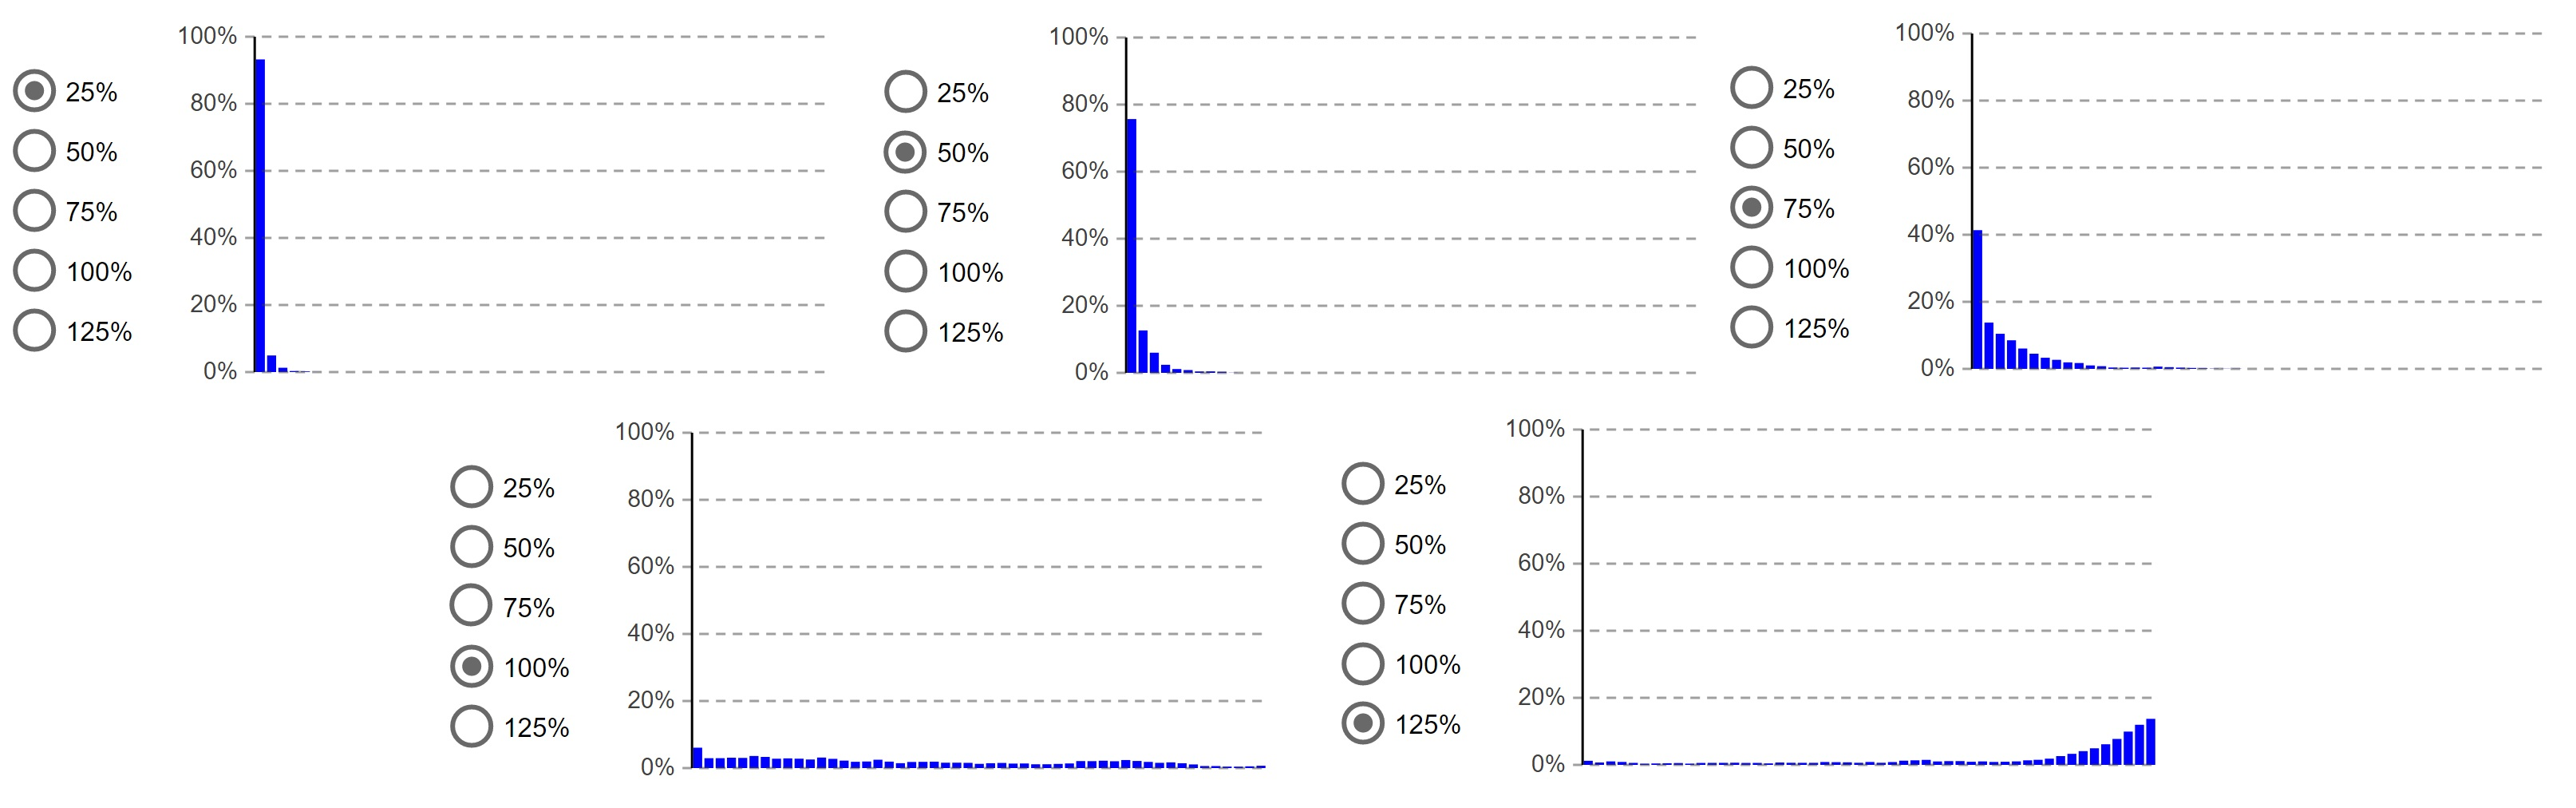
\includegraphics[width=\linewidth]{images/anylogic-colas-50}
  \caption{Probabilidad de encontrar n clientes en cola.}
\end{figure}

